\subsection{Analysis}
%Partition algorithm is the main part of both insertion
%and detection algorithms. Time complexity $\T$ is related to number of edges 
%$|E|$ in map and the ratio of partition threshold $\theta$ to total road length
%$\LEN=\sum_{R \in M}length(R)$. %$\theta$ should be a constant, which sets a threshold 
%for the algorithm how much information a subregion should contain at least to embed 
%a one bit watermark. 
The time complexity of \algoref{Partition} is 
\[\T = O(|E|\log\LEN),\]
where $\LEN$ is the total length of all roads in map $M$.
%A digital road map $M$ is a special case of a connected graph 
%$G=\left\{V,~E\right\}$.
%A general connected graph has the following constraints on $|E|$ and $|V|$.
%\[|V|-1 \le |E|\le \frac{|V|(|V|-1)}{2}.\]
%which means in the worse case of a fully connected graph, 
%However, in practice, map graphs are much more sparse. In fact, 
%every vertex is either the end of a road, a turning point of a road or a junction. 
Since the number of edges connected to a vertex is bounded a small number $q$, 
that is, $|E| \le (q\times|V|)/2$, $\T = O(|V|\log\LEN)$.
%Considering the practical situation, the number of intersecting vertices is 
%insignificant comparing to $|E|$. On other hand, to control the cost, the
%intersecting vertices of roads in real world are also weakly connected. 
%Then we have a good reason to assume that $|E| \cong |V|$. 

The time complexity of \algoref{algo:Insertion} and \algoref{algo:Detection} 
%$PO$ is a list of $submap$. 
%We can distinguish all watermarking points by traversing it. 
is $\T+O(|V|)$, or $O(|V|\log\LEN)$.

%a watermarking process must guarantee a low false positive rate. 
%That means that it should maintain low rate of detecting 
%unwatermarked data as watermarked data.
The detection confidence in (\ref{eqn:conf})
essentially represents the probability of correctly identifying watermarks 
in a given map (attacked or not). We now attempt to give a lower bound
to the detection confidence. 
%, so it is possible for the 
%algorithm to detect an unwatermarked map as ``illegal''
%In order to avoid discovering watermark from data not marked, 
%we define detection accuracy$(DA)$. 
Intuitively, as $\theta$ decreases, the map is divided into more
subregions and therefore more watermarks will be inserted while
the accuracy of watermark detection should be enhanced. We thus have
the following lemma.
%Furthermore, to resell the digital map, an attack should firstly keep 
%the usability of the map not 
%only in accuracy degradation but also in size of the map. For example, if the map of 
%Minnesota state is watermarked and published. An attacker who wants to resell part of 
%this map may prefer to crop a sub-map of a county from the whole map. Thus the partition 
%algorithm should partition a county map into enough sub-regions. Meanwhile, since the watermark 
%is inserted at an arbitrary (hashed) bit position of a vertex's x-coordinate, it can be 
%either ``0'' or ``1'' with almost equal probability. We obtain Lemma \ref{lemm}.
\begin{lemma}
\label{lemma-accuracy}
Given a map $M$ with total length $\LEN$ and an algorithm threshold $\theta$, 
the minimum detection confidence for $M$: 
\[
\label{pe}
conf_{min}(M) = 1 - \sum _{ i={\lceil\rho\LEN/{4 \theta}\rceil} }^{ \lceil\LEN/{4 \theta}\rceil}
{{\lceil \LEN/{4 \theta}\rceil \choose i} {\left(\frac{1}{2}\right)}^{\lceil \LEN/{4 \theta}\rceil}} 
\]
where $\rho$ is the ratio between the number of leaf nodes that match and
the total number of leaf nodes in $M$. 
\end{lemma}
\begin{proof}
Straightforward as the total number of leaf nodes is no less than $\LEN/{4 \theta}$.
\end{proof}

\begin{figure}[h]
\centering
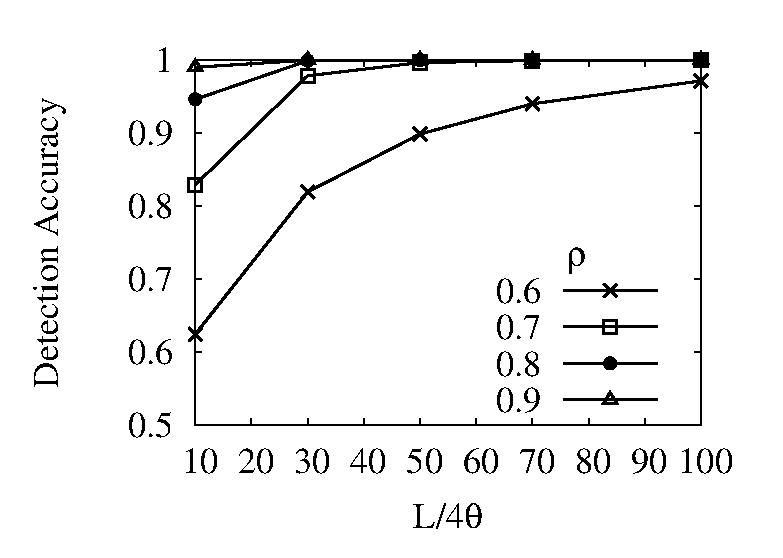
\epsfig{file=images/security.eps,width=0.6\columnwidth}
\caption{Accuracy of Detection}
\label{fig:security}
\end{figure} 

\figref{fig:security} plots the relationship between minimum detection confidence 
against $\LEN/4\theta$ for different values of $\rho$, which coincides with our
previous intuition.
However, smaller $\theta$ translates into more watermarks and hence larger
distortion to the map. It also causes the watermarking to be more 
time-consuming. This trade-off should be carefully considered when applying our
approach.

